\documentclass[11pt]{article}
%
%
% Retirez le caractere "%" au debut de la ligne ci-dessous si votre
% editeur de texte utilise des caracteres accentues
% \usepackage[latin1]{inputenc}
\setlength{\headheight}{14pt}
%
% Retirez le caractere "%" au debut des lignes ci-dessous si vous
% utiisez les symboles et macros de l'AMS
 \usepackage{amsmath}
\usepackage{amsfonts}
\usepackage{amsthm}
\newtheorem{lemma}{Lemma}
\newtheorem{proposition}{Proposition}
\newtheorem{remark}{Remark}

\usepackage{fancyhdr}
\pagestyle{fancy}
\fancyhead{}
\usepackage{graphicx}
\usepackage{color}

%\usepackage{biblatex}
%\addbibresource{Biblio.bib}

\usepackage[left=2.5cm,right=2.5cm,top=2.5cm,bottom=2.5cm]{geometry}
\setlength{\parskip}{6pt}
\usepackage{lmodern}
\usepackage[T1]{fontenc}
\usepackage[utf8]{inputenc}
\usepackage[english]{babel}
%\usepackage{caption}


\usepackage{amsopn}             % pour \DeclareMathOperator
\usepackage{amssymb}            % pour \leqslant
\usepackage{algorithmicx}
%\usepackage{algorithm2e}
\usepackage{algorithm}
\usepackage{algpseudocode}

\DeclareMathOperator{\cov}{cov}
\DeclareMathOperator{\cor}{cor}
\DeclareMathOperator{\var}{var}
\DeclareMathOperator{\sign}{sign}
\DeclareMathOperator{\sumss}{SS}
\DeclareMathOperator{\diag}{diag}
\DeclareMathOperator{\rank}{rank}
\DeclareMathOperator*{\argmin}{arg\,min}
\DeclareMathOperator*{\argmax}{arg\,max}
\DeclareMathOperator*{\minimize}{minimize}
\DeclareMathOperator{\trace}{\mathrm{trace}}
\DeclareMathOperator{\vMF}{vMF}
\DeclareMathOperator{\Ga}{Gamma}
\DeclareMathOperator{\Bern}{Bernoulli}
\DeclareMathOperator{\Be}{Beta}

\newcommand{\X}{\mathbf{X}}
\newcommand{\U}{\mathbf{U}}
\newcommand{\V}{\mathbf{V}}
\newcommand{\EE}{\mathbf{E}}
\newcommand{\HH}{\mathbf{H}}
\newcommand{\F}{\mathbf{F}}
\newcommand{\W}{\mathbf{W}}
\newcommand{\Q}{\mathbf{Q}}
\newcommand{\uu}{\mathbf{u}}
\newcommand{\vv}{\mathbf{v}}
\newcommand{\ww}{\mathbf{w}}
\newcommand{\f}{\mathbf{f}}
\newcommand{\z}{\mathbf{z}}
\newcommand{\I}{\mathbf{I}}
\newcommand{\one}{\mathbf{1}}
\newcommand{\Stiefel}[2]{\mathcal V_{#1,#2}}



\begin{document}
\renewcommand{\headrulewidth}{0pt}


%--------------------------------------------------------------------------

\begin{center}
{\Large
	{\sc Bayesian Framework for Canonical factorization of multiblock data}
}
\bigskip

 %\underline{Jean-Michel Galharret}$^{1}$ \& Stephanie Bougeard $^{2}$ \& Katrijn Van Deun$^{3}$ \& Mohamed Hanafi$^{1}$
\bigskip

%{\it
%$^{1}$ Oniris, INRAE, StatSC, Nantes, France. \\
%$^{2}$ Epidemiology and Welfare, ANSES, Ploufragan, France. \\
%$^{3}$ Department of Methodology and Statistics, Tilburg University, Tilburg, The Netherlands.
%}
\end{center}
\bigskip

--------------------------------------------------------------------------

\section{Introduction}

Data sets structured into blocks of variables measured on the same set of observations are frequently encountered in practice. These blocks may consist of quantitative variables originating from distinct measurement sources or correspond to thematic groupings defined by the user. For instance, in omics studies, blocks typically comprise variables derived from different analytical techniques (e.g., proteomics, metabolomics). In psychology, multiblock data structures commonly arise when multiple sets of variables are collected on the same individuals to capture different psychological domains. For example, distinct blocks may include self-report questionnaire scores assessing personality traits, behavioral task performance measures, and neurophysiological indicators such as electroencephalography  features.

The four expected objectives of exploratory multiblock data analysis are: (i) to perform a joint dimensionality reduction, (ii) to examine relationships among blocks, (iii) to investigate associations among variables both within and across blocks, and (iv) to capture within-block variability in order to reveal shared and block-specific structures in a common latent space.  An unified algebraic framework based on factorization strategies, denoted \textit{canonical factorisation}, was proposed by \cite{bougeard2024} for multiblock methods to achieve these objectives. In practice, canonical factorisation provides a structured framework for analysing data variability at multiple levels: differences between and within blocks, differences between observations by projecting them onto a common subspace. It also facilitates the harmonisation of outputs produced by different methods and supports a more objective criterion-based selection among competing approaches. 
The four expected objectives of exploratory multiblock data analysis are: (i) to perform a joint dimensionality reduction, (ii) to examine relationships among blocks, (iii) to investigate associations among variables both within and across blocks, and (iv) to capture within-block variability in order to reveal shared and block-specific structures in a common latent space.  An unified algebraic framework based on factorization strategies, denoted \textit{canonical factorisation}, was proposed by \cite{bougeard2024} for multiblock methods to achieve these objectives. In practice, canonical factorisation provides a structured framework for analysing data variability at multiple levels: differences between and within blocks, differences between observations by projecting them onto a common subspace. It also facilitates the harmonisation of outputs produced by different methods and supports a more objective criterion-based selection among competing approaches. 

%This framework is a compass among multiblock models:  Generalized Canonical Correlation Analysis (GCCA, \cite{Carroll68}) and its popular case MAXVAR \cite{Carroll68}, Hierarchical Principal Component Analysis (HPCA, \cite{Wold96,Westerhuis98}), Structuration de Tableaux A Tois Indices de la Statistique (Statis, \cite{Lavit94}), Multiple Factorial Analysis (MFA, \cite{escofier1994}), Common Components and Specific Weights Analysis (CCWSA, \cite{Qannari001}), Multiple CO-inertia Analysis (MCOA, \cite{Chessel96})  fall within this framework. A benchmark of these methods had been done in \cite{Bougeard024}.

%Initially, MCOA was proposed as an alternative to generalized canonical analysis, also known as MAXVAR \cite{Carroll68,Horst59}, for correlating multiple data tables. Compared with other generalisations of Hotelling's canonical correlation analysis \cite{Hotelling35}, such as those proposed by \cite{Kettenring71}, MCOA offers three main advantages. Firstly, it is computationally straightforward as it reduces to a singular value decomposition, the other approaches typically rely on iterative optimisation procedures. Secondly, MCOA is particularly effective at summarizing results across multiple datasets. Finally, MCOA provides sequential estimation of canonical factorisation under an orthogonality constraint.  In this work, we propose a new method, Optimal Multiple CO-inertia Analysis (OMCOA), which is a simultaneous version of MCOA. We compare this model with the previous one using simulated data whose structure is known.     

\section{Canonical factorisation}
\subsection*{Notations}

\begin{itemize}
	\item $K$ blocks  $(\textbf{X}_1,\ldots,\textbf{X}_K)$ respectively of $p_1,\ldots,p_K$ variables on $N$ individuals,
	\item  $\textbf{X}=[\textbf{X}_1|\ldots|\textbf{X}_K]\in \mathcal M_{N,P}(\mathbb R)$ ($P=\sum_{k=1}^K p_k$) be the concatenation of these $K$-blocks,
	\item $\textbf{U}^\intercal$ designates the transposed matrix of $\textbf{U}$, 
	\item $\Sigma_k=diag(\sigma_k^{(1)},...,\sigma_k^{(R)})$ are diagonal matrices 
	\item $\Vert . \Vert$ correspond to the Frobenius norm,
	\item $\Stiefel{N}{R}=\{\W\in\mathcal M_{N,R}(\mathbb R):\W^\intercal\W=\I_R\}$
denotes the Stiefel manifold.
\end{itemize}
 
Consider $K$ colmumn blocks  $(\textbf{X}_1,\ldots,\textbf{X}_K)$ respectively in $\mathcal M_{N,p_1}(\mathbb R),...,\mathcal M_{N,p_K}(\mathbb R))$. Let $\textbf{X}=[\textbf{X}_1|\ldots|\textbf{X}_K]\in \mathcal M_{N,P}(\mathbb R)$ ($P=\sum_{k=1}^K p_k$) be the concatenation of these $K$-blocks. Without loss of generality, the blocks are assumed to be column-centered.

\cite{bougeard2024} demonstrated that the $(K+1)-$blocks $(\textbf{X}_1,\ldots,\textbf{X}_K,\textbf{X})$ can be factorized in dimension $R=rank(\textbf{X})$ as follows  
\begin{align}
  \left\{
	\begin{array}{ll}
		&\X   = \U \Sigma \V^\intercal   \\
		&\X_k = \U \Sigma_k \V_k^\intercal \quad \textrm{for} \quad k=(1, \dots, K)    \\	
		&\textrm{with the constraints} \quad \U\in \Stiefel{N}{R} \quad \textrm{and} \quad \Vert\vv_k^{(1)}\Vert=\ldots=\Vert\vv_k^{(R)}\Vert=1 \quad \textrm{for} \quad k=(1, \dots, K), 
	\end{array}
	\right. \label{Cano_Facto}
\end{align}
where
\begin{itemize}
	\item $\U\in \Stiefel{N}{R}$ is the block-common components,
	\item $\V_k \in \mathcal M_{p_k,R}(\mathbb R)$ are the  block-loadings, and $\V=[\V_1|...|\V_K] \in \mathcal M_{P,R}(\mathbb R)$,
  \item $\Sigma\in \mathcal M_{R,R}(\mathbb R)$ the diagonal scaling matrices with property $\Sigma^2 = \sum_{k=1}^K \Sigma_k^2$ that relate common and block-analyses.
\end{itemize}
Without loss of generality, we can assume $\sigma_k^{(r)}\geq 0$ for all $k,r$, since a joint sign change of $\sigma_k^{(r)}$ and $\vv_k^{(r)}$ leaves the model and the constraints unchanged. Since the blocks $\X_1,...\X_K$ are column-centered, the block-common $\U\in\Stiefel{N}{R}$ is centered as-well:
$$\U\in\Stiefel{N}{R}, \quad \mathbf{1}_N\U=0.$$
This factorization is \textit{the canonical factorization}. Each multiblock method derives a common component $\U$ using a different optimization criterion. Projecting the data onto these common components enables their canonical factorization (for details see \cite{bougeard2024}). For all the multiblock methods, once $\U$ is fixed, the decomposition $\X_k=\U\Sigma_k\V_k^\intercal$ of each block is unique (up to sign). The methods differ in how the axes $\uu^{(1)},\ldots,\uu^{(R)}$ themselves are determined. When the block loadings are only normalized ($\|\vv_k^{(r)}\|=1$), the optimal loadings are
$\vv_k^{(r)}=\X_k^\intercal\uu^{(r)}/\|\X_k^\intercal\uu^{(r)}\|$ and the least-squares criterion reduces to
\[
  \sum_{k=1}^K\bigl\|\X_k-\U\Sigma_k\V_k^\intercal\bigr\|^2=\|\X\|^2-\bigl\|\X^\intercal\U\bigr\|^2 ,
\]
which is invariant under any rotation $\U\mapsto\U\mathbf R$: only $\mathrm{span}(\U)$ is determined by the data, and the axes have to be fixed by an external convention, usually the SVD of $\X$. This convention becomes unstable when the singular values of $\X$ are close. When $\V_k\in\Stiefel{p_k}{R}$ for all $k$, the criterion is no longer rotation invariant, and the axes of $\U$ are identified (up to permutation and sign) by the block-specific profiles $\Sigma_1,\ldots,\Sigma_K$, as long as these profiles differ across blocks. 
 
%For $R<rank(\textbf{X})$, the objective is to determine the optimal approximation of the form given in \eqref{Cano_Facto} by minimizing an ordinary least square criterion.    

\subsection{Canonical Factorisation under orthogonal block-loadings constraint}

Providing a solution for canonical factorization means minimizing
\begin{equation}
	\sum_{k=1}^K\Vert \X_k - \U\Sigma_k \V_k^\intercal\Vert^2= \Vert \X- \U \Sigma \V^\intercal\Vert^2, \label{Crit}
\end{equation}
with $\U\in\Stiefel{N}{R}$, $\V_k\in\Stiefel{p_k}{N}$ for $k=1,\ldots,K$. 
%Note that, with standardized and orthogonal block-loadings matrices $\V_1,\ldots,\V_K$, the solution of this problem is unique. 
Chessel and Hanafi \cite{chessel1996} proposed a sequential solution, known as Multiple Co-Inertia Analysis (MCOA): the dimensions are computed one at a time, each from the blocks deflated with respect to the previous block loadings. This procedure yields orthonormal matrices $\U$ and $\V_1,\ldots,\V_K$, and each stage is optimal in the
least-squares sense given the previous ones. The resulting solution is nevertheless suboptimal with respect to \eqref{Crit}, since each dimension is chosen without taking the next ones into account, so that the $R$ dimensions are not fitted simultaneously.
Optimal Multiple COinertia Ananlysis (OMCOA) is proposed as a simultaneous solution of \eqref{Crit} under the constraints $\U\in \Stiefel{N}{R}$ and $\V_k\in \Stiefel{N}{R}$ ($k=1,\ldots,K$). It is computed by an alternating least squares (ALS) algorithm, in which each step minimizes \eqref{Crit} with respect to one set of parameters, the others being fixed:
\begin{itemize}
  \item \textbf{Update of $\U$:} $\U=\mathbf A\mathbf B^\intercal$, where $\X\mathbf H^\intercal=\mathbf A\mathbf D\mathbf B^\intercal$ is the SVD of
        $\X\mathbf H^\intercal$, with $\mathbf H=[\Sigma_1\V_1^\intercal|\cdots|\Sigma_K\V_K^\intercal]$ (orthogonal Procrustes problem);
  \item \textbf{Update of $\V_k$:} $\V_k=\mathbf A_k\mathbf B_k^\intercal$, where $\X_k^\intercal\U\Sigma_k=\mathbf A_k\mathbf D_k\mathbf B_k^\intercal$
        is the SVD of $\X_k^\intercal\U\Sigma_k$, for $k=1,\ldots,K$;
  \item \textbf{Update of $\Sigma_k$:} $\Sigma_k=\diag(\U^\intercal\X_k\V_k)$, for $k=1,\ldots,K$.
\end{itemize}
%These steps are iterated until the decrease of \eqref{Crit} falls below a given tolerance. Since each step cannot increase the criterion, which is bounded below, the sequence of criterion values converges; 

\begin{proposition}
  The successive updates of $\U,\V_k,\Sigma_k$ guarantee that the criterion defined in \eqref{Crit} decreases or remains constant at each step, ensuring convergence of the algorithm.  
\end{proposition}
The proof is given in the appendix.
\begin{remark}
Since the limit may however be a local minimum, the algorithm is started from the MCOA solution and from several random initializations, and the solution with the lowest criterion is retained.  
\end{remark}



\section{Bayesian framework for Canonical Factorisation}

A probabilistic counterpart of \eqref{Crit} is obtained by assuming a Gaussian noise:
\begin{equation}
  \X_k=\U\Sigma_k\V_k^\intercal+\EE_k,\qquad
  \EE_k\ \sim \ \mathcal N\bigl(0,\tau_k^{-1}\bigr),\qquad k=1,\ldots,K,
  \label{eq:model}
\end{equation}
where $\tau_k$ is the noise precision of block $k$. %Since the blocks are centered, the latent components are constrained to be
centered as well: $\U\in\Stiefel{N}{R}$ with $\one_N^\intercal\U=0$.

\paragraph{Priors.} We use the following independent priors:
\begin{itemize}
  \item $\U$ and $\V_1,\ldots,\V_K$ are uniformly distributed on their Stiefel manifolds (non-informative von Mises--Fisher distribution). A random matrix $\W\in\Stiefel{m}{R}$ follows the matrix von Mises--Fisher distribution $\vMF(\F)$, with parameter $\F\in\mathcal M_{m,R}(\mathbb R)$, if its density with
respect to the uniform measure on $\Stiefel{m}{R}$ is proportional to $\exp\{\trace(\F^\intercal\W)\}$
\cite{hoff2009}. If $\F=\mathbf A\mathbf D\mathbf B^\intercal$ is the SVD of $\F$, the mode of $\vMF(\F)$ is the
polar factor $\mathbf A\mathbf B^\intercal$, and the distribution concentrates around it as the singular values of $\F$ increase.
  \item $\sigma_k^{(r)}\sim\mathcal N^+\bigl(0,\lambda^{-1}\bigr)$, a half-normal distribution with a small precision
        $\lambda$ (e.g.\ $\lambda=10^{-2}$); 
  \item $\tau_k\sim\Ga(a_0,b_0)$ with small hyperparameters (e.g.\ $a_0=b_0=10^{-3}$).
\end{itemize}

\subsection{Full conditional distributions}

\paragraph{Likelihood.} Because $\U$ and $\V_k$ have orthonormal columns and $\Sigma_k$ is diagonal,
\begin{equation}
  \bigl\|\X_k-\U\Sigma_k\V_k^\intercal\bigr\|^2
  =\|\X_k\|^2-2\trace\bigl(\Sigma_k\V_k^\intercal\X_k^\intercal\U\bigr)+\sum_{r=1}^R\bigl(\sigma_k^{(r)}\bigr)^2 .
  \label{eq:expand}
\end{equation}
Since the blocks are centered, each $\X_k$ carries $(N-1)p_k$ degrees of freedom, and the log-likelihood is
\[
  \log p(\X_1,\ldots,\X_K\mid\cdot)=\sum_{k=1}^K\Bigl[\tfrac{(N-1)p_k}{2}\log\tau_k
  -\tfrac{\tau_k}{2}\bigl\|\X_k-\U\Sigma_k\V_k^\intercal\bigr\|^2\Bigr]+\text{const}.
\]
By \eqref{eq:expand}, $\U$ and $\V_k$ only appear in the linear term $\trace(\Sigma_k\V_k^\intercal\X_k^\intercal\U)$.
This is the key property: all the full conditionals belong to standard families.



\begin{proposition}[Full conditionals]\label{prop:cond}
Under model \eqref{eq:model} and the above priors:
\begin{enumerate}
  \item \textbf{Common space.} Let $\Q\in\mathcal M_{N,N-1}(\mathbb R)$ be an orthonormal basis of
        $\one_N^\perp$ and write $\U=\Q\tilde\U$ with $\tilde\U\in\Stiefel{N-1}{R}$. Then
        \[
          \tilde\U\mid\cdot\ \sim\ \vMF\bigl(\Q^\intercal\F_{\U}\bigr),\qquad
          \F_{\U}=\sum_{k=1}^K\tau_k\,\X_k\V_k\Sigma_k .
        \]
  \item \textbf{Block loadings.} For $k=1,\ldots,K$,
        \[
          \V_k\mid\cdot\ \sim\ \vMF\bigl(\F_{\V_k}\bigr),\qquad \F_{\V_k}=\tau_k\,\X_k^\intercal\U\Sigma_k .
        \]
  \item \textbf{Block weights.} For $k=1,\ldots,K$ and $h=1,\ldots,H$, let $d_k^{(r)}={\uu^{(r)}}^\intercal\X_k\vv_k^{(r)}$. Then
        \[
          \sigma_k^{(r)}\mid\cdot\ \sim\ \mathcal N^+\Bigl(\frac{\tau_k\,d_k^{(r)}}{\tau_k+\lambda},\ \frac{1}{\tau_k+\lambda}\Bigr),
        \]
        a normal distribution truncated to $(0,+\infty)$.
  \item \textbf{Noise precisions.} For $k=1,\ldots,K$,
        \[
          \tau_k\mid\cdot\ \sim\ \Ga\Bigl(a_0+\frac{(N-1)p_k}{2},\ b_0+\frac{1}{2}\bigl\|\X_k-\U\Sigma_k\V_k^\intercal\bigr\|^2\Bigr).
        \]
\end{enumerate}
\end{proposition}
\noindent The modes of the full conditionals of Proposition~\ref{prop:cond} are
\[
  \U=\mathbf A\mathbf B^\intercal\ \text{with}\ \F_{\U}=\mathbf A\mathbf D\mathbf B^\intercal,\qquad
  \V_k=\mathbf A_k\mathbf B_k^\intercal\ \text{with}\ \F_{\V_k}=\mathbf A_k\mathbf D_k\mathbf B_k^\intercal,\qquad
  \sigma_k^{(h)}=\frac{\tau_k}{\tau_k+\lambda}\,d_k^{(h)} .
\]
When $\lambda\to0$ and the precisions are equal ($\tau_1=\cdots=\tau_K$), these are exactly the OMCOA updates:
Procrustes rotation of $\X\mathbf H^\intercal$ for $\U$ (with $\mathbf H=[\Sigma_1\V_1^\intercal|\cdots|\Sigma_K\V_K^\intercal]$),
Procrustes rotation of $\X_k^\intercal\U\Sigma_k$ for $\V_k$, and $\Sigma_k=\diag(\U^\intercal\X_k\V_k)$. OMCOA is therefore the iterated conditional modes (ICM) algorithm \cite{besag1986} associated with this posterior, and the Gibbs sampler is its
stochastic counterpart. With block-specific precisions, $\F_{\U}=\sum_k\tau_k\X_k\V_k\Sigma_k$ weights each block by its estimated noise precision, so that noisier blocks contribute less to the common space. To reproduce exactly the OMCOA criterion \eqref{Crit}, a common precision $\tau_1=\cdots=\tau_K=\tau$ can be used, with
\eqref{Crit},
$\tau\mid\cdot\sim\Ga\bigl(a_0+\sum_k(N-1)p_k/2,\ b_0+\sum_k\|\X_k-\U\Sigma_k\V_k^\intercal\|^2/2\bigr)$.

\paragraph{Post-processing: label switching and signs}\label{sec:align}

The posterior distribution is invariant under any permutation $\pi$ of the $R$ dimensions applied jointly to
$\U$, $\V_1,\ldots,\V_K$ and $\Sigma_1,\ldots,\Sigma_K$, and under a joint change of sign of $\uu^{(r)}$ and
$\vv_1^{(r)},\ldots,\vv_K^{(r)}$. Posterior summaries are therefore computed after aligning each draw on a reference
$\U_{\mathrm{ref}}$ (in practice the OMCOA solution). For each draw, with $\mathbf C=\U_{\mathrm{ref}}^\intercal\U$,
\[
  \hat\pi=\argmax_{\pi\in\mathfrak S_R}\sum_{h=1}^R\bigl|C_{r,\pi(r)}\bigr|,\qquad
  s_r=\operatorname{sign}\bigl(C_{r,\hat\pi(r)}\bigr),
\]
and the columns of $\U$ and $\V_k$ are reordered by $\hat\pi$ and multiplied by $s_r$, while the diagonal of
$\Sigma_k$ is reordered by $\hat\pi$ (it stays positive). Posterior means and credible intervals of $\sigma_k^{(r)}$
are then obtained from the empirical distribution of the aligned draws.

We can deduce the following algorithm:

\begin{algorithm}[ht]
\caption{Gibbs sampler for OMCOA}\label{alg:gibbs}
\begin{algorithmic}[1]
  \Require centered blocks $\X_1,\ldots,\X_K$; dimension $H$; number of iterations $T$; burn-in $T_0$;
           hyperparameters $a_0,b_0,\lambda$
  \State \textbf{Initialization:} $\U=\Q\tilde\U$, $\V_k$, $\Sigma_k$ from OMCOA (or MCOA, or at random);
         $\tau_k\gets(N-1)p_k\big/\|\X_k-\U\Sigma_k\V_k^\intercal\|^2$
  \For{$t=1,\ldots,T$}
     \State $\F_{\U}\gets\sum_{k}\tau_k\,\X_k\V_k\Sigma_k$;\quad update $\tilde\U$ by one column-wise sweep of $\vMF(\Q^\intercal\F_{\U})$;\quad $\U\gets\Q\tilde\U$
     \For{$k=1,\ldots,K$}
        \State $\F_{\V_k}\gets\tau_k\,\X_k^\intercal\U\Sigma_k$;\quad update $\V_k$ by one column-wise sweep of $\vMF(\F_{\V_k})$
        \For{$h=1,\ldots,H$}
           \State $d_k^{(h)}\gets{\uu^{(h)}}^\intercal\X_k\vv_k^{(h)}$;\quad draw
                  $\sigma_k^{(h)}\sim\mathcal N^+\bigl(\tau_kd_k^{(h)}/(\tau_k+\lambda),\,1/(\tau_k+\lambda)\bigr)$
        \EndFor
        \State draw $\tau_k\sim\Ga\bigl(a_0+(N-1)p_k/2,\ b_0+\|\X_k-\U\Sigma_k\V_k^\intercal\|^2/2\bigr)$
     \EndFor
     \If{$t>T_0$} store $\bigl(\U,\V_1,\ldots,\V_K,\Sigma_1,\ldots,\Sigma_K,\tau_1,\ldots,\tau_K\bigr)$ \EndIf
  \EndFor
  \State \textbf{Post-processing:} align each stored draw on a reference solution (Section~\ref{sec:align})
  \State \Return the aligned draws
\end{algorithmic}
\end{algorithm}

% \begin{remark}[What the sampler adds]
% Besides point estimates close to the OMCOA solution, the sampler provides the posterior distribution of the block
% weights $\sigma_k^{(h)}$ and of the noise levels $\tau_k^{-1}$. Credible intervals on $\sigma_k^{(h)}$ can be used to assess
% whether a dimension is common to all blocks, shared by some of them, or specific to one block.
% \end{remark}

% \begin{remark}[Practical aspects]
% Starting from the OMCOA solution shortens the burn-in. The column-wise sweeps make successive draws of $\U$ and
% $\V_k$ correlated, so convergence should be checked on trace plots of the $\sigma_k^{(h)}$. Because the posterior is
% strongly concentrated when the noise is small, the chain rarely jumps between the $H!$ equivalent modes; the alignment step
% remains necessary nonetheless, in particular when several dimensions have close weights.
% \end{remark}

\section{Sparse Bayesian Framework for canonical factorisation}
In OMCOA, each block is approximated as $\X_k\approx\U\Sigma_k\V_k^\intercal$, where the diagonal matrix
$\Sigma_k=\diag(\sigma_k^{(1)},\ldots,\sigma_k^{(R)})$ measures how much each latent dimension $\uu^{(r)}$ contributes to
block $k$. The structure of the blocks can be read from the pattern of zeros of $\Sigma_1,\ldots,\Sigma_K$: dimension
$r$ is
\begin{itemize}
  \item \emph{$U$-common} if $\sigma_k^{(r)}>0$ for all $k$;
  \item \emph{partially $U$-common} if $\sigma_k^{(r)}>0$ for some blocks only;
  \item \emph{$U$-specific} to block $k$ if $\sigma_k^{(r)}>0$ for this block only;
  \item \emph{inactive} if $\sigma_k^{(r)}=0$ for all $k$.
\end{itemize}
OMCOA always returns strictly positive weights, so that this pattern has to be assessed afterwards. We propose
a Bayesian version of OMCOA in which a spike-and-slab prior on the weights $\sigma_k^{(r)}$ allows them to be exactly
zero. The dimension $R$ is then a \emph{maximal} rank: inactive dimensions are switched off by the sampler, and the
effective rank is inferred from the data.

The sparsity of the model is based on the diagonal terms $\sigma_k^{(r)}$ as follows
\begin{equation}
  \sigma_k^{(r)}=\gamma_k^{(r)}\,s_k^{(r)},\qquad \gamma_k^{(r)}\in\{0,1\},\quad s_k^{(r)}>0 .
  \label{eq:spike}
\end{equation}

\paragraph{Priors.} The difference between the two sets of prior distributions lies in the prior distributions of the diagonal terms: 
\begin{itemize}
  \item spike-and-slab on the weights:
        $\gamma_k^{(r)}\mid\theta_r\sim\Bern(\theta_r)$ and $s_k^{(r)}\sim\mathcal N^+(0,\lambda^{-1})$, i.e.\
        \[
          p\bigl(\sigma_k^{(r)}\mid\theta_r\bigr)=(1-\theta_r)\,\delta_0\bigl(\sigma_k^{(r)}\bigr)+\theta_r\,\mathcal N^+\bigl(\sigma_k^{(r)};0,\lambda^{-1}\bigr);
        \]
  \item $\theta_r\sim\Be(a_\theta,b_\theta)$, one inclusion probability per dimension, shared by the $K$ blocks.
\end{itemize}
Sharing $\theta_r$ across blocks borrows strength: a dimension that is active in several blocks is more likely
to be active in another one, and a dimension that is inactive everywhere sees $\theta_r$ shrink towards zero.

As in the non-sparse case, the orthonormality of $\U$ and $\V_k$ gives
\begin{equation}
  \bigl\|\X_k-\U\Sigma_k\V_k^\intercal\bigr\|^2=\|\X_k\|^2-2\sum_{r=1}^R\sigma_k^{(r)}d_k^{(r)}+\sum_{r=1}^R\bigl(\sigma_k^{(r)}\bigr)^2,
  \qquad d_k^{(r)}={\uu^{(r)}}^\intercal\X_k\vv_k^{(r)} .
  \label{eq:expand2}
\end{equation}

\begin{proposition}[Full conditionals]\label{prop:cond2}
Let $\Q\in\mathcal M_{N,N-1}(\mathbb R)$ be an orthonormal basis of $\one_N^\perp$ and write $\U=\Q\tilde\U$.
\begin{enumerate}
  \item \textbf{Common space:} $\tilde\U\mid\cdot\sim\vMF(\Q^\intercal\F_{\U})$ with $\F_{\U}=\sum_k\tau_k\X_k\V_k\Sigma_k$.
  \item \textbf{Block loadings:} $\V_k\mid\cdot\sim\vMF(\F_{\V_k})$ with $\F_{\V_k}=\tau_k\X_k^\intercal\U\Sigma_k$.
        When $\sigma_k^{(r)}=0$, the $r$-th column of $\F_{\V_k}$ is zero and $\vv_k^{(r)}$ is uniform on the orthogonal
        complement of the other columns.
  \item \textbf{Weights (joint update of $\gamma_k^{(r)}$ and $\sigma_k^{(r)}$).} Let
        \[
          \omega_k=\tau_k+\lambda,\qquad m_k^{(r)}=\frac{\tau_k\,d_k^{(r)}}{\omega_k}.
        \]
        Then, with $\sigma_k^{(r)}$ integrated out,
        \[
          P\bigl(\gamma_k^{(r)}=1\mid\cdot\bigr)=\frac{\theta_r B_k^{(r)}}{\theta_rB_k^{(r)}+1-\theta_r},\qquad
          B_k^{(r)}=2\sqrt{\frac{\lambda}{\omega_k}}\,
          \exp\Bigl(\frac{\omega_k\bigl(m_k^{(r)}\bigr)^2}{2}\Bigr)\,\Phi\Bigl(m_k^{(r)}\sqrt{\omega_k}\Bigr),
        \]
        where $\Phi$ is the standard normal c.d.f.; and
        \[
          \sigma_k^{(r)}\mid\gamma_k^{(r)}=1,\cdot\ \sim\ \mathcal N^+\bigl(m_k^{(r)},\omega_k^{-1}\bigr),\qquad
          \sigma_k^{(r)}\mid\gamma_k^{(r)}=0,\cdot\ =\ 0 .
        \]
  \item \textbf{Inclusion probabilities:}
        $\theta_r\mid\cdot\sim\Be\bigl(a_\theta+\sum_k\gamma_k^{(r)},\ b_\theta+K-\sum_k\gamma_k^{(r)}\bigr)$.
  \item \textbf{Noise precisions:}
        $\tau_k\mid\cdot\sim\Ga\bigl(a_0+(N-1)p_k/2,\ b_0+\|\X_k-\U\Sigma_k\V_k^\intercal\|^2/2\bigr)$.
\end{enumerate}
\end{proposition}


Updating $(\gamma_k^{(r)},\sigma_k^{(r)})$ jointly, with $\sigma_k^{(r)}$ integrated out when drawing $\gamma_k^{(r)}$, is essential:
drawing $\gamma_k^{(r)}$ given the current $\sigma_k^{(r)}$ would never allow the chain to leave $\sigma_k^{(r)}=0$.
In practice $\log B_k^{(r)}$ is computed on the log scale, with $\log\Phi$ evaluated directly, to avoid overflow.


%The matrix von Mises--Fisher distributions are sampled by one column-wise sweep per iteration, each column being drawn from a vector von Mises--Fisher distribution with Wood's algorithm, as in the non-sparse sampler.

We can deduce the following algorithm:

\begin{algorithm}[ht]
\caption{Sparse Gibbs sampler for OMCOA}\label{alg:sparse}
\begin{algorithmic}[1]
  \Require centered blocks $\X_1,\ldots,\X_K$; maximal rank $R\leq\min_kp_k$; iterations $T$; burn-in $T_0$;
           hyperparameters $a_0,b_0,\lambda,a_\theta,b_\theta$
  \State \textbf{Initialization:} $\U,\V_k,\Sigma_k$ from OMCOA with $R$ dimensions; $\gamma_k^{(r)}\gets1$; $\theta_r\gets1/2$;
         $\tau_k\gets(N-1)p_k\big/\|\X_k-\U\Sigma_k\V_k^\intercal\|^2$
  \For{$t=1,\ldots,T$}
     \State update $\tilde\U$ by one sweep of $\vMF\bigl(\Q^\intercal\sum_k\tau_k\X_k\V_k\Sigma_k\bigr)$;\quad $\U\gets\Q\tilde\U$
     \For{$k=1,\ldots,K$}
        \State update $\V_k$ by one sweep of $\vMF\bigl(\tau_k\X_k^\intercal\U\Sigma_k\bigr)$
        \For{$r=1,\ldots,R$}
           \State $d_k^{(r)}\gets{\uu^{(r)}}^\intercal\X_k\vv_k^{(r)}$,\quad $\omega_k\gets\tau_k+\lambda$,\quad $m_k^{(r)}\gets\tau_kd_k^{(r)}/\omega_k$
           \State draw $\gamma_k^{(r)}\sim\Bern\Bigl(\dfrac{\theta_rB_k^{(r)}}{\theta_rB_k^{(r)}+1-\theta_r}\Bigr)$
           \State \textbf{if} $\gamma_k^{(r)}=1$ \textbf{then} draw $\sigma_k^{(r)}\sim\mathcal N^+\bigl(m_k^{(r)},\omega_k^{-1}\bigr)$ \textbf{else} $\sigma_k^{(r)}\gets0$
        \EndFor
        \State draw $\tau_k\sim\Ga\bigl(a_0+(N-1)p_k/2,\ b_0+\|\X_k-\U\Sigma_k\V_k^\intercal\|^2/2\bigr)$
     \EndFor
     \For{$r=1,\ldots,R$}
        \State draw $\theta_r\sim\Be\bigl(a_\theta+\sum_k\gamma_k^{(r)},\ b_\theta+K-\sum_k\gamma_k^{(r)}\bigr)$
     \EndFor
     \If{$t>T_0$} store $\bigl(\U,\Sigma_1,\ldots,\Sigma_K,\boldsymbol\gamma,\boldsymbol\theta,\boldsymbol\tau\bigr)$ \EndIf
  \EndFor
  \State align the stored draws (permutation and signs) on a reference $\U_{\mathrm{ref}}$
  \State \Return the aligned draws
\end{algorithmic}
\end{algorithm}

From the posterior distributions of the parameter $\gamma_k^{(r)}$ a decision rule for the representation of the block $\X_k$ on the component $u^{(r)}$: 
\begin{quote} 
  the component $\uu^{(r)}$ is active for the block $k$ if and only if $P(\gamma_k^{(r)}=1\mid\X_1,\ldots,\X_K)>1/2$. 
\end{quote}
\noindent Moreover, this model makes it possible to estimate the rank of the blocks $(\X_1,...,\X_K)$ i.e. $R_{\mathrm{eff}}=\#\{r:\sum_k\gamma_k^{(r)}>0\}$, whose posterior distribution is estimated by its empirical distribution over the draws. 




% \begin{lemma} \label{lemma1}
% 	For given matrices $\X\in\mathcal M_{N,P}(\mathbb R),\h\in\mathcal M_{P,R}(\mathbb R)$, the maximum of $\trace(\T^\intercal\X\h)$ with the constraint $\T^\intercal.\T=I_R$ is $\T=\textbf{U}.\textbf{V}^\intercal$ where the columns of $\textbf{U}$ (respectively $\textbf{V}$) are the $R$ first left (respectively right) singular vectors of $\X\h$. (see \cite{cliff66}) 
% \end{lemma}

% \begin{proof}
% 	Consider the SVD of $\X.\h =\textbf{U}.\Sigma.\textbf{V}^t$. We have $\trace(\textbf{T}^t.\textbf{U}.\Sigma.\textbf{V}^t)=\trace(\Sigma.\textbf{V}^t.\textbf{T}^t.\textbf{U})$
% 	($\trace(\textbf{A}.\textbf{B})=\trace(\textbf{B}.\textbf{A})$). The matrix $\textbf{W}=\textbf{V}^t.\textbf{T}^t.\textbf{U}$ is orthogonal. 
% The problem of maximization remains to maximizing 
% \[\trace(\Sigma.\textbf{W})=\sum_{h=1}^H\sigma^2_h.w_{hh}.\]
% Since $\textbf{W}$ is orthogonal, $|w_{hh}| \leq 1$ for all $h$. The trace of $\Sigma.\textbf{W}$ is maximal for $w_{hh}=1$, that implies $\textbf{W}=I_H$ and $\textbf{T}=\textbf{U}.\textbf{V}^t$. Moreover, the maximum of the trace is  $\sum_{h=1}^H\sigma^2_h$. 

% \end{proof}

% \begin{lemma} \label{lemma2}
% 	For given matrices $\X\in\mathcal M_{N,P}(\mathbb R),\h\in\mathcal M_{P,R}(\mathbb R), \T \in \mathcal M_{N,R}(\mathbb R)$ we have 
% 	\[\trace(\textbf{X}^\intercal.\textbf{T}.\textbf{H}^\intercal)=\trace(\textbf{T}^\intercal\textbf{X}\textbf{H}).\]
% \end{lemma}

%  \begin{proof}
%  $\trace(\X^\intercal\T\h^\intercal)=\trace(\h^\intercal\X^\intercal\T)=\trace(\T^\intercal\X\h).$
%  The first equality comes from $\trace(\textbf{A}\textbf{B})=\trace(\textbf{A}\textbf{B})$ for $\textbf{A},\textbf{B}$ of dimension $N,P$ and $P,N$. The second equality comes from the equality of the trace of a square matrix and its transpose.
%  \end{proof}


% \medskip
% \noindent
% \textbf{Remark.} This proof guarantees convergence of the values of the criterion, but not necessarily uniqueness of the limit point. Uniqueness of the solution is established separately, via the orthogonality of the columns of $\V_k$ for all $k$.

% \section{Comparison of MCOA and OMCOA}
% \subsection{Simulation study}
% MCOA and OMCOA are compared on simulated data. $K=3$ blocks $\X_1,\X_2,\X_3$ with respectively
% $p_1=10$, $p_2=15$, $p_3=20$ variables and $N=100$ observations are generated from
% \[
% \X_k=\U\Sigma_k\V_k^\intercal+\EE_k, \qquad k=1,2,3,
% \]
% where $\U\in\mathcal M_{N,R}(\mathbb R)$ (column-centered) and $\V_k\in\mathcal M_{p_k,R}(\mathbb R)$ have orthonormal
% columns, $R=3$, $\Sigma_k$ is diagonal and $\EE_k$ is a Gaussian noise term.
% We compare the estimation of $\Sigma_1,\ldots,\Sigma_K$ obtained with MCOA and OMCOA.
% The diagonal matrices depend on a parameter $t\in[0,1]$:
% \[
% \Sigma_k(t)=(1-t)\,\Sigma^{(0)}_k+t\,\Sigma_k^{(1)},
% \]
% where
% \begin{itemize}
%   \item for $t=0$, all the blocks share the same profile:
%   $\Sigma^{(0)}_1=\Sigma^{(0)}_2=\Sigma^{(0)}_3=\diag(0.7,\,0.5,\,0.3)$;
%   \item for $t=1$, each block has its own dominant dimension of the common space $\U$ (permuted profiles):
%   $\Sigma^{(1)}_1=\diag(0.7,\,0.5,\,0.3)$, $\Sigma^{(1)}_2=\diag(0.5,\,0.3,\,0.7)$, $\Sigma^{(1)}_3=\diag(0.3,\,0.7,\,0.5)$.
% \end{itemize}
% In both cases $\sum_{r}(\sigma_k^{(r)})^2=0.83$ for each block. Moreover, the singular values of the
% noise-free concatenated matrix are $\bigl(\sum_k(\sigma_k^{(r)}(t))^2\bigr)^{1/2}$: they are well separated for $t=0$
% and all equal to $\sqrt{0.83}$ for $t=1$, since $\sum_k\Sigma_k^{(1)\,2}=0.83\,\textbf{I}_3$.
% The noise is scaled so that $\|\EE_k\|^2=\frac{0.10}{0.90}\,\|\U\Sigma_k\V_k^\intercal\|^2$, i.e.\ it accounts for about
% $10\%$ of the variance of each block. We use $t\in\{0,0.1,\ldots,1\}$ and $B=1000$ replications.

% At each replication, the estimated axes are reordered by the permutation
% \[
% \hat\pi=\arg\max_{\pi\in\mathfrak S_R}\sum_{r=1}^{R}\bigl|\cos\bigl(\u^{(r)},\hat\u^{(\pi(r))}\bigr)\bigr|,
% \]
% the absolute value accounting for the sign indeterminacy of the axes.
% The accuracy of the estimation of $\Sigma_1,\ldots,\Sigma_K$ is assessed by the mean absolute error
% over the $K$ blocks and the $R$ dimensions:
% \[
% \mathrm{MAE}=\frac{1}{KR}\sum_{k=1}^{K}\sum_{r=1}^{R}
% \bigl|\hat\sigma_k^{(\hat\pi(r))}-\sigma_k^{(r)}\bigr|.
% \]

% \subsection{Results}

% \begin{figure}
%   \centering
%   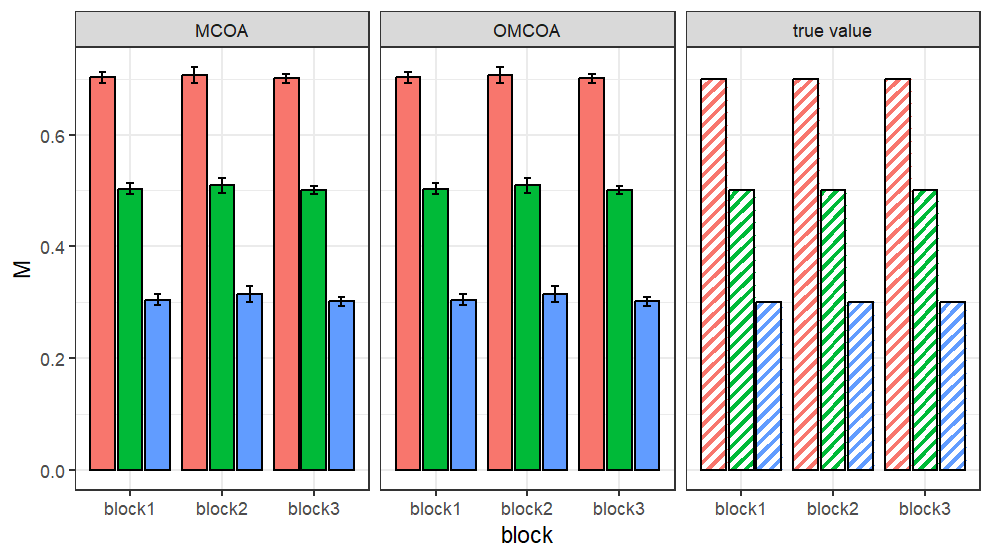
\includegraphics[width=.8\linewidth]{figs/plot_t0.png}
%   \caption{Common profile ($t=0$): median and 10--90\% empirical quantiles of $\hat\sigma^{(\hat\pi(r))}_k$
%   over the $B=1000$ replications (red: dim~1, green: dim~2, blue: dim~3).\label{fig_t0}}
% \end{figure}

% \begin{figure}
%   \centering
%   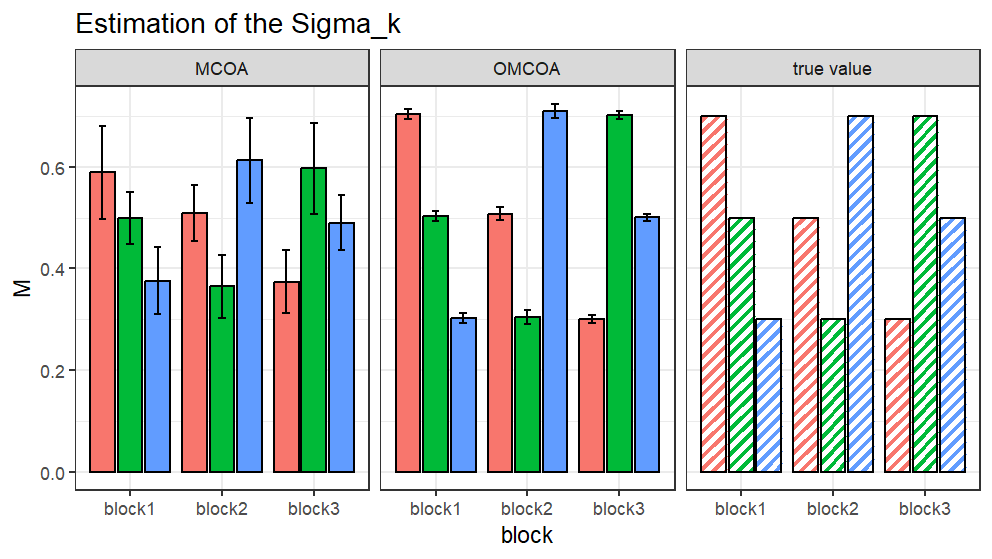
\includegraphics[width=.8\linewidth]{figs/plot_t1.png}
%   \caption{Permuted profiles ($t=1$): median and 10--90\% empirical quantiles of $\hat\sigma^{(\hat\pi(r))}_k$
%   over the $B=1000$ replications (red: dim~1, green: dim~2, blue: dim~3).\label{fig_t1}}
% \end{figure}

% Figures~\ref{fig_t0} and~\ref{fig_t1} show the estimates obtained with MCOA and OMCOA for $t=0$ and $t=1$
% respectively. As expected, both methods give very close estimates when the blocks share a common profile
% (Figure~\ref{fig_t0}). When the profiles are permuted, OMCOA outperforms MCOA in terms of both bias and
% precision (Figure~\ref{fig_t1}). In both scenarios, the OMCOA estimates show very low variability.

% \begin{figure}
%   \centering
%   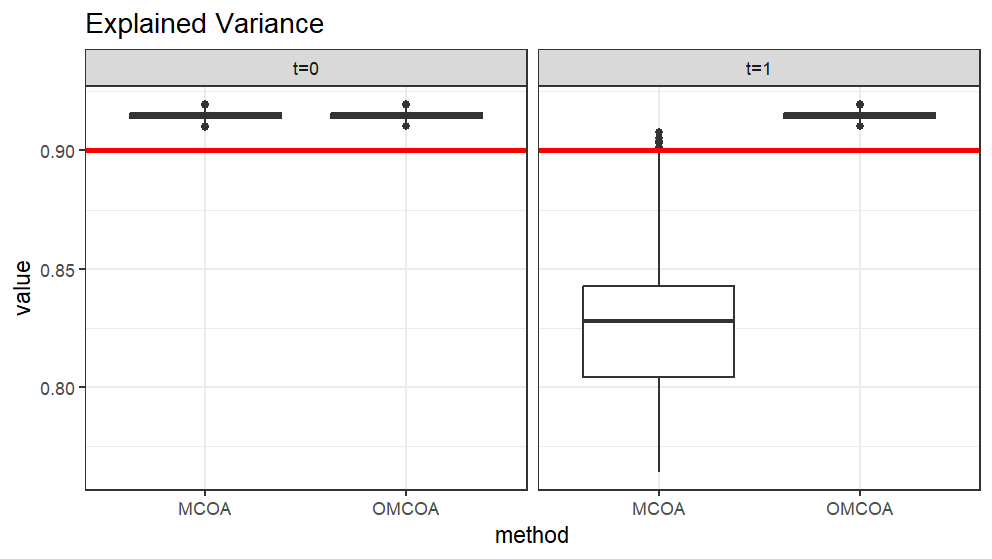
\includegraphics[width=.8\linewidth]{figs/explained_var.png}
%   \caption{Distribution of the percentage of explained variance $V$ over the $B=1000$ replications.\label{var_expl}}
% \end{figure}

% Figure~\ref{var_expl} shows the empirical distribution of the percentage of variance of the concatenated
% matrix $\X$ explained by the $R$ dimensions,
% \[
% V=100\times\frac{\sum_{k,r}\bigl(\hat\sigma^{(r)}_k\bigr)^2}{\|\X\|^2},
% \qquad \|\X\|^2=\sum_{k=1}^{K}\|\X_k\|^2,
% \]
% to be compared with the percentage of variance due to the signal, which is about $90\%$ by construction.
% OMCOA slightly exceeds this value in all cases, since part of the noise is captured by the fitted
% dimensions, whereas MCOA clearly underestimates it when the profiles are permuted ($t=1$).

% Figure~\ref{comparison_t} shows the distribution of the MAE as a function of $t$. MCOA and OMCOA coincide as
% long as the singular values of $\X$ are well separated; MCOA breaks down when they get close ($t\geq 0.8$).
% Indeed, MCOA starts with the SVD of $\X$: when the singular values are close, $\u^{(1)}$ is an arbitrary
% direction of $\mathrm{span}(\U)$ driven by the noise, and this error propagates to the next dimensions through
% the deflation. OMCOA fits all the blocks simultaneously, so that the block-specific profiles identify $\U$.
% Figure~\ref{comparison_cos} illustrates the resulting misestimation of the axes $\u^{(1)},\ldots,\u^{(R)}$
% by MCOA for $t\geq 0.8$.

% \begin{figure}
%   \centering
%   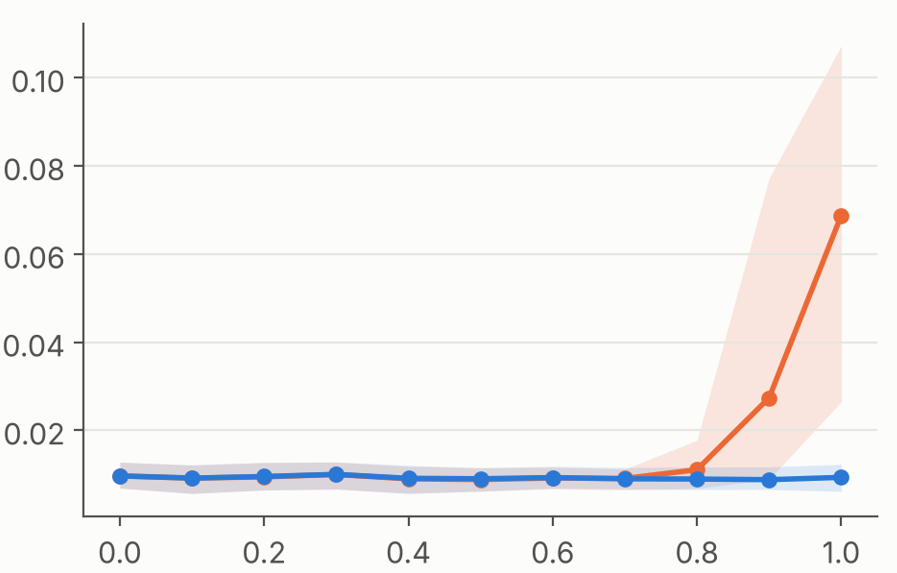
\includegraphics[width=.5\linewidth]{figs/comparaison_t.png}
%   \caption{Median and 10--90\% empirical quantiles of the MAE as a function of $t$ ($B=1000$ replications).\label{comparison_t}}
% \end{figure}

% \begin{figure}
%   \centering
%   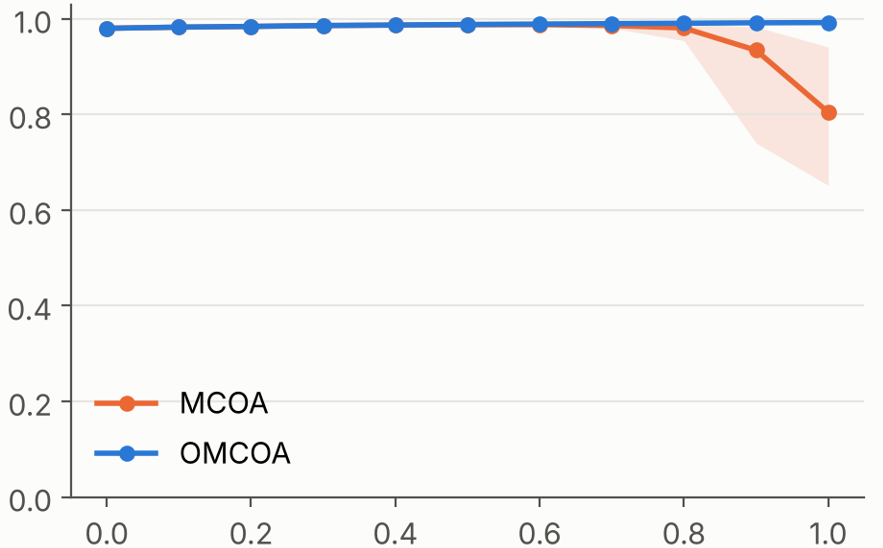
\includegraphics[width=.5\linewidth]{figs/comparaison_cos.png}
%   \caption{Median and 10--90\% empirical quantiles of the worst axis recovery
%   $\displaystyle\min_{r}\bigl|\cos\bigl(\u^{(r)},\hat\u^{(\hat\pi(r))}\bigr)\bigr|$ as a function of $t$
%   ($B=1000$ replications).\label{comparison_cos}}
% \end{figure}

% \section*{Conclusion}
% \cite{Bougeard024} have compared estimations for the canonical factorisation problem. In this work, we propose on optimal version of Multiple COinertia Analysis that performs better on the simulated data. Constraining the matrices $(\V_1,\dots,\V_K)$ to be orthogonal ensures uniqueness of the solution. In particular, if $|\mathbf{E}_k|=0$, the OMCOA method recovers the exact canonical factorization while other methods do not guarantee this."    
% Furthermore, in practical applications the canonical factorisation is more readily interpreted under orthogonal configurations, as these yield a clearer decomposition of the effects.




\bibliographystyle{apalike}
\bibliography{Biblio}

\section*{Appendix: proof of the proposition}


\begin{proof}
	The criterion to be minimized is:
\[
  \mathcal{L}(\U, \V_1, \ldots, \V_K, \Sigma_1, \ldots, \Sigma_K)
  = \sum_{k=1}^{K} \bigl\| \X_k - \U \Sigma_k \V_k^\top \bigr\|^2,
\]
subject to $\U^\intercal \U = I_R$ and $\V_k^\intercal \V_k = I_R$ for all $k = 1, \ldots, K$.

The algorithm is of the \emph{Alternating Least Squares} (ALS) type: at each iteration, the criterion is minimized successively with respect to each parameter, while the others are held fixed. It therefore suffices to show that each individual update decreases or maintains $\mathcal{L}$.

\paragraph{Update of $\U$} With $\V_k$ and $\Sigma_k$ fixed, let $\HH_k = \Sigma_k \V_k^\intercal \in \mathcal{M}_{R,p_k}(\mathbb{R})$ and
$\HH = [\HH_1 \mid \cdots \mid \HH_K] \in \mathcal{M}_{R,P}(\mathbb{R})$. Then:
\[
  \mathcal{L} = \sum_{k=1}^{K} \|\X_k - \U \HH_k\|^2 = \|\X - \U \HH^\intercal\|^2.
\]
Expanding:
$\|\X - \U \HH^\intercal\|^2
  = \|\X\|^2 - 2\,\operatorname{trace}(\X^\intercal \U \HH^\intercal) + \|\U \HH^\intercal\|^2.$

\noindent Since $\U^\intercal \U = I_R$: $\|\U \HH^\intercal\|^2
  = \operatorname{trace}(\HH \U^\intercal \U \HH^\intercal)
  = \operatorname{trace}(\HH \HH^\intercal)
  = \|\HH\|^2 \quad \text{(constant w.r.t.\ } \U\text{)}.$

\noindent Minimizing $\mathcal{L}$ with respect to $\U$ is therefore equivalent to
maximizing $$\trace(\X^\intercal\U\HH^\intercal)=\trace(\HH^\intercal\X^\intercal\U)=\trace(\U^\intercal\X\HH),$$
subject to $\U^\intercal \U = I_R$. The first equality comes from $\trace(\textbf{A}\textbf{B})=\trace(\textbf{A}\textbf{B})$ for $\textbf{A},\textbf{B}$ of dimension $N,P$ and $P,N$. The second equality comes from the equality of the trace of a square matrix and its transpose. By \cite{cliff1966}, the maximum is attained at $\U^* = AB^\intercal$, where $A$ (resp.\ $B$) are the matrices of the $R$ leading left (resp.\ right) singular vectors of $\X\HH^T$.
subject to $\U^\intercal \U = I_R$. The first equality comes from $\trace(\textbf{A}\textbf{B})=\trace(\textbf{A}\textbf{B})$ for $\textbf{A},\textbf{B}$ of dimension $N,P$ and $P,N$. The second equality comes from the equality of the trace of a square matrix and its transpose. By \cite{cliff1966}, the maximum is attained at $\U^* = AB^\intercal$, where $A$ (resp.\ $B$) are the matrices of the $R$ leading left (resp.\ right) singular vectors of $\X\HH^T$.
This update is the global minimizer of $\mathcal{L}$ with respect to $\U$, hence:
\[
  \mathcal{L}(\U^*, \ldots) \leq \mathcal{L}(\U_{\mathrm{old}}, \ldots).
\]
\paragraph{Update of $\V_k$} With $\U$ and $\Sigma_k$ fixed, expanding the contribution of block $k$:
\[
  \|\X_k - \U \Sigma_k \V_k^\intercal\|^2
  = \|\X_k\|^2
    - 2\,\operatorname{trace}(\X_k^\intercal \U \Sigma_k \V_k^\intercal)
    + \|\U \Sigma_k \V_k^\intercal\|^2.
\]
Since $\U^\intercal \U = I_R$ and $\V_k^\intercal \V_k = I_R$:
\[
  \|\U \Sigma_k \V_k^\intercal\|^2
  = \operatorname{trace}(\V_k \Sigma_k^\intercal \U^\intercal \U \Sigma_k \V_k^\intercal)
  = \operatorname{trace}(\Sigma_k^2)
  \quad \text{(constant w.r.t.\ } \V_k\text{)}.
\]
Minimizing therefore reduces to maximizing
$\operatorname{trace}(\X_k^\intercal \U \Sigma_k \V_k^\intercal) = \operatorname{trace}(\V_k^\intercal\X_k^\intercal\U\Sigma_k)$
subject to $\V_k^\intercal \V_k = I_R$. Since the diagonal matrix $\Sigma_k > 0$ does not affect the singular vectors, the maximum is attained at $\V_k^* = \textbf{AB}^\intercal$ where $\textbf{A}$, $\textbf{B}$ are obtained from the SVD of $\X_k^\intercal\U$ \cite{cliff1966} . Hence:
subject to $\V_k^\intercal \V_k = I_R$. Since the diagonal matrix $\Sigma_k > 0$ does not affect the singular vectors, the maximum is attained at $\V_k^* = \textbf{AB}^\intercal$ where $\textbf{A}$, $\textbf{B}$ are obtained from the SVD of $\X_k^\intercal\U$ \cite{cliff1966} . Hence:
\[
  \mathcal{L}(\ldots, \V_k^*, \ldots) \leq \mathcal{L}(\ldots, \V_{k,\mathrm{old}}, \ldots).
\]

%---------------------------------------------------------------
\paragraph{Update of $\Sigma_k$} With $\U$ and $\V_k$ fixed (both having orthonormal columns), and $\Sigma_k = \operatorname{diag}(\sigma^{(1)}_k,
\ldots, \sigma^{(R)}_k)$, the contribution of block $k$ is:
\[
  \|\X_k - \U \Sigma_k \V_k^\intercal\|^2
  = \|\X_k\|^2
    - 2\,\operatorname{trace}(\V_k^\intercal \X_k^\intercal \U \Sigma_k)
    + \operatorname{trace}(\Sigma_k^2).
\]
Since $\Sigma_k$ is diagonal, it remains to minimazing:
\[
  \sum_{r=1}^{R} \Bigl[ ()\sigma^{(r)}_k)^2 - 2\,(\U^\intercal \X_k \V_k)_{rr} \cdot d_r \Bigr].
\]
Each term is a convex parabola in $\sigma^{(r)}_k$, minimized at: $(\sigma^{(r)}_k)^* = (\U^\intercal \X_k \V_k)_{rr},$ or, in matrix form:$\Sigma_k^* = \operatorname{diag}(\U^\intercal \X_k \V_k).$
This update is therefore the exact minimizer with respect to $\Sigma_k$, and:
\[
  \mathcal{L}(\ldots, \Sigma_k^*, \ldots) \leq \mathcal{L}(\ldots, \Sigma_{k,\mathrm{old}}, \ldots).
\]

%---------------------------------------------------------------
\paragraph{Global Convergence} At each complete iteration (update of $\U$, then all $\V_k$, then all $\Sigma_k$), the criterion $\mathcal{L}$ is monotonically decreasing and bounded below by zero. By the monotone convergence theorem, the sequence of values $(\mathcal{L}^{(t)})_{t \geq 0}$
converges:
\[
  \mathcal{L}^{(t+1)} \leq \mathcal{L}^{(t)}, \quad \mathcal{L}^{(t)} \geq 0
  \implies
  \mathcal{L}^{(t)} \xrightarrow[t \to \infty]{} \ell^* \geq 0.
\]
\end{proof}

\begin{proof}[Sketch of proof]
(1)--(2): by \eqref{eq:expand}, the conditional density of $\U$ is proportional to
$\exp\{\sum_k\tau_k\trace(\Sigma_k\V_k^\intercal\X_k^\intercal\U)\}=\exp\{\trace(\F_{\U}^\intercal\U)\}$, and
$\trace(\F_{\U}^\intercal\Q\tilde\U)=\trace\bigl((\Q^\intercal\F_{\U})^\intercal\tilde\U\bigr)$; the same argument applies to $\V_k$
with $\trace(\Sigma_k\V_k^\intercal\X_k^\intercal\U)=\trace(\F_{\V_k}^\intercal\V_k)/\tau_k$.
(3): the terms of \eqref{eq:expand} involving $\sigma_k^{(h)}$ are $-\frac{\tau_k}{2}\bigl[(\sigma_k^{(h)})^2-2\sigma_k^{(h)}d_k^{(h)}\bigr]$;
adding the log-prior $-\frac{\lambda}{2}(\sigma_k^{(h)})^2$ and completing the square gives a Gaussian kernel, restricted to
$\sigma_k^{(h)}>0$.
(4): the Gamma prior is conjugate for the precision of a Gaussian likelihood.
\end{proof}

\paragraph{Sampling from the matrix von Mises--Fisher distribution}
Direct sampling from $\vMF(\F)$ is not straightforward, but its column-wise conditionals are vector von
Mises--Fisher distributions \cite{hoff2009}. Let $\W_{-j}$ be $\W$ without its $j$-th column and
$\mathbf N_j\in\mathcal M_{m,m-H+1}(\mathbb R)$ an orthonormal basis of $\mathrm{span}(\W_{-j})^\perp$. Then
\[
  \ww_j=\mathbf N_j\z,\qquad \z\sim\vMF\bigl(\mathbf N_j^\intercal\f_j\bigr)\ \text{on the unit sphere } \mathbb S^{m-H},
\]
where $\f_j$ is the $j$-th column of $\F$. One sweep over the $H$ columns (in random order) is a valid Gibbs update
of $\W$, which is enough inside the Gibbs sampler. The vector distribution $\vMF(\f)$, with density
proportional to $\exp(\f^\intercal\z)$ on $\mathbb S^{m-1}$, is sampled with the rejection algorithm of Wood \cite{wood1994}
(Algorithm~\ref{alg:wood}).

\begin{algorithm}[ht]
\caption{Sampling $\z\sim\vMF(\f)$ on $\mathbb S^{m-1}$ (Wood, 1994)}\label{alg:wood}
\begin{algorithmic}[1]
  \State $\kappa\gets\|\f\|$,\quad $\boldsymbol\mu\gets\f/\kappa$
  \State $b\gets (m-1)\big/\bigl(2\kappa+\sqrt{4\kappa^2+(m-1)^2}\bigr)$,\quad $x_0\gets(1-b)/(1+b)$,\quad
         $c\gets\kappa x_0+(m-1)\log(1-x_0^2)$
  \Repeat
     \State draw $\zeta\sim\mathrm{Beta}\bigl(\tfrac{m-1}{2},\tfrac{m-1}{2}\bigr)$ and $\upsilon\sim\mathcal U(0,1)$
     \State $w\gets\bigl(1-(1+b)\zeta\bigr)\big/\bigl(1-(1-b)\zeta\bigr)$
  \Until{$\kappa w+(m-1)\log(1-x_0w)-c\geq\log\upsilon$}
  \State draw $\boldsymbol\xi\sim\mathcal N(\mathbf 0,\I_m)$, set $\boldsymbol\xi\gets\boldsymbol\xi-(\boldsymbol\mu^\intercal\boldsymbol\xi)\boldsymbol\mu$
         and $\boldsymbol\xi\gets\boldsymbol\xi/\|\boldsymbol\xi\|$
  \State \Return $\z=w\,\boldsymbol\mu+\sqrt{1-w^2}\,\boldsymbol\xi$
\end{algorithmic}
\end{algorithm}

\noindent The expression of $b$ used in Algorithm~\ref{alg:wood} is algebraically equivalent to Wood's original one,
$b=\bigl(-2\kappa+\sqrt{4\kappa^2+(m-1)^2}\bigr)/(m-1)$, but avoids a numerical cancellation when $\kappa$ is large,
which is the typical situation here since $\kappa$ scales with the noise precisions $\tau_k$.

\begin{proof}[Sketch of proof]
Items 1, 2, 4 and 5 follow as in the non-sparse sampler (linearity of \eqref{eq:expand} in $\U$ and $\V_k$, and
conjugacy). For item 3, the terms of the log-posterior involving $\sigma_k^{(r)}$ are, by \eqref{eq:expand},
$\tau_kd_k^{(r)}\sigma_k^{(r)}-\frac{\tau_k}{2}(\sigma_k^{(r)})^2$. Under $\gamma_k^{(r)}=0$, $\sigma_k^{(r)}=0$ and this quantity is
$0$. Under $\gamma_k^{(r)}=1$, integrating against the half-normal slab of density
$2\sqrt{\lambda/(2\pi)}\exp(-\lambda s^2/2)$ on $(0,\infty)$ gives
\[
  2\sqrt{\frac{\lambda}{2\pi}}\int_0^{\infty}\exp\Bigl(-\frac{\omega_k}{2}s^2+\tau_kd_k^{(r)}s\Bigr)ds
  =2\sqrt{\frac{\lambda}{\omega_k}}\exp\Bigl(\frac{\omega_k(m_k^{(r)})^2}{2}\Bigr)\Phi\bigl(m_k^{(r)}\sqrt{\omega_k}\bigr)=B_k^{(r)},
\]
which is the Bayes factor of $\gamma_k^{(r)}=1$ against $\gamma_k^{(r)}=0$. The conditional of $\sigma_k^{(r)}$ given
$\gamma_k^{(r)}=1$ is obtained by completing the square.
\end{proof}



%\printbibliography




% \subsection{Multiple CO-Inertia Analysis}
% \cite{Chessel96} proposed Multiple Co-inertia Analysis as an alternative to MAXVAR \cite{Carroll68}. The rank-$H$ approximation is derived from successive rank-1 approximations of deflated versions of the blocks $\X_1,\ldots,\X_K$.

% The rank-1 approximation criterion is based on minimising the sum of squared Frobenius norms
% \begin{equation}
%     \sum_{k=1}^K\Vert \X_k - \sigma_{k}\u\v_k^\intercal \Vert^2, \quad \Vert \u\Vert = \Vert \v_1\Vert = \ldots = \Vert \v_K\Vert = 1, \quad \sigma_k > 0. \label{mcoa_c}
% \end{equation}

% \noindent The solution to this minimisation problem is:
% \begin{itemize}
%   \item $\u$ is the first left singular vector of the concatenated block $\X$,
%   \item $\v_k = \frac{\X_k^\intercal \u}{\Vert \X_k^\intercal \u \Vert}$,
%   \item $\sigma_k = \Vert \X_k^\intercal \u \Vert$ for $k = 1, \ldots, K$.
% \end{itemize}
 

% The algorithm proposed by \cite{Chessel96} proceeds as follows: at each step $r = 1, \ldots, R$, the rank-1 approximation is applied to the deflated blocks $\X_k^{(r)} = \X_k(I_{p_k}-\sum_{i=1}^{r-1}\v_k^{(i)}{\v_k^{(i)}}^\intercal)$. Moreover, they proved that the resulting vectors $\u^{(1)}, \ldots, \u^{(R)}$ are mutually orthogonal. Note that, thanks to the deflation procedure,  $\v_k^{(1)}, \ldots, \v_k^{(R)}$ are mutually orthogonal for each $k$.
% MCOA belongs to the class of sequential multiblock component methods. In the first stage, the global
% component $\u^{(1)}$ and the block loadings $\v_1^{(1)},\ldots,\v_K^{(1)}$ are obtained as the solution of a least-squares criterion; the next dimensions are then computed in the same way from deflated versions of the original blocks. Although each stage is optimal in the least-squares sense given the previous ones, the sequential approach is sub-optimal: the resulting solution does not minimize the global criterion
% \eqref{Crit} over the $H$ dimensions simultaneously. The present study proposes a simultaneous alternative to MCOA, which minimizes \eqref{Crit} under the same orthonormality constraints on $\V_1,\ldots,\V_K$.



\end{document}

